\chapter{Neutron Transport Theory}{\label{ch:Neutron Transport Theory}
    %%% Continuous Energy quantities %%%
% Cross-sections
\DeclareDocumentCommand{\xst}{ O{\loc} O{E} }{\ensuremath{\CrossSection_{t}(#1,#2)}}
\DeclareDocumentCommand{\xsa}{ O{\loc} O{E} }{\ensuremath{\CrossSection_{a}(#1,#2)}}
\DeclareDocumentCommand{\xsf}{ O{\loc} O{\Eprime} }{\ensuremath{\CrossSection_{f}(#1,#2)}}
\DeclareDocumentCommand{\xss}{ o O{\loc} O{\dirprime\vdot\dir} O{\Eprime \to E}}{
    \IfNoValueOrEmptyTF{#1}
    {\ensuremath{\CrossSection_{s}(#2,#3,#4)}}
    {\ensuremath{\CrossSection_{s,#1}(#2,#4)}}
}
\DeclareDocumentCommand{\spect}{ O{\loc} O{E} }{\ensuremath{\Spectrum(#1,#2)}}
\DeclareDocumentCommand{\nufis}{ O{\loc} O{E^{\prime}} }{ \ensuremath{\nu\xsf[#1][#2] }}

% Flux
\DeclareDocumentCommand{\aflux}{ O{\loc} O{\dir} O{E} }{\ensuremath{\AngularFlux(#1,#2,#3)}}
\DeclareDocumentCommand{\sflux}{ O{\loc} O{E} }{\ensuremath{\ScalarFlux(#1,#2)}}
\DeclareDocumentCommand{\current}{ O{\loc} O{E} }{\ensuremath{\Current(#1,#2)}}
\DeclareDocumentCommand{\afluxmom}{ O{\loc} O{E} O{\ell} O{n} }{\FluxMoment^{#4}_{#3}(#1,#2)}

% Source
\DeclareDocumentCommand{\source}{ O{\loc} O{\dir} O{E} }{\ensuremath{Q(#1,#2,#3)}}
   % Continuous space, direction, and energy quantities
    \def\figpath{chapters/02/figures/}
    \graphicspath{ {\figpath} }

    In this chapter, the basic theory behind the neutron transport equation, and the numerical methods used to solve it are introduced.

    \section{Neutron Transport Equation}{\label{sec:NTT:Neutron Transport Equation}
        The fundamental equation for all neutron transport methods is the neutron transport equation:
        \begin{aequation}\label{eq:NTT:Boltzmann Transport}
                &\Big[\frac{1}{v(E)}\pderiv{}{t} + \dir\vdot\grad + \xst[\loc][E,t]\Big]\aflux[\loc][\dir][E,t]
                    = \\&\qquad\qquad
                    \rfourpi\Bigg[
                        \source[\loc][\dir][E,t]\\&\qquad\qquad
                        + \intl[0][\infty]\intl[\fourpi]\xss[][\loc][\dirprime\vdot\dir][\Eprime\to E,t]\aflux[\loc][\dirprime][\Eprime,t]\ddirprime\dif{\Eprime}\\&\qquad\qquad
                        + \spect\intl[0][\infty]\nufis[\loc][\Eprime,t]\intl[\fourpi]\aflux[\loc][\dirprime][\Eprime,t]\ddirprime\dif{\Eprime}
                    \Bigg],
        \end{aequation}
        \begin{equation*}
            \forall\loc, \quad \forall\dir\in\fourpi,\quad \forall E\in[0,\infty),\quad \forall t\geq 0,
        \end{equation*}
        where $\loc$ is the location vector, $\dir$ is the direction vector, $E$ is the neutron energy, $t$ is the time, $v$ is the neutron velocity, $\CrossSection$ quantities are the cross sections, $\AngularFlux$ is the angular flux, $\nu$ is the average number of neutrons produced per fission, and $\Spectrum$ is the fission spectrum.

        The location vector, $\loc$, is a column vector of the spatial coordinates:
        \begin{equation}\label{eq:NTT:Location Vector}
            \loc \defined \begin{bmatrix}x\\y\\z\end{bmatrix}.
        \end{equation}
        The direction vector, $\dir$, is a column unit-vector which gives the direction of flight for neutrons, and is defined by
        \begin{subequations}\label{eqs:NTT:Direction Definitions}
            \begin{equation}\label{eq:NTT:Direction Vector}
                \dir \defined
                    \begin{bmatrix}
                        \Direction_x\\\Direction_y\\\Direction_z
                    \end{bmatrix}
                    =
                    \begin{bmatrix}
                        \sqrt{1-\PolarCos^2}\cos(\Azimuthal)\\
                        \sqrt{1-\PolarCos^2}\sin(\Azimuthal)\\
                        \PolarCos
                    \end{bmatrix},
            \end{equation}
            where $\Azimuthal$ is the azimuthal angle, and $\PolarCos$ is the cosine of the polar angle $\Polar$,
            \begin{equation}\label{eq:NTT:Polar Cosine}
                \PolarCos \defined \cos(\Polar).
            \end{equation}
        \end{subequations}
        This spatial and angular coordinates system is depicted visually in \cref{fig:NTT:Transport Coordinate System}.

        \begin{figure}[h]
            \centering
            \def\svgwidth{0.4\linewidth}
            \input{\figpath/TransportCoordinateSystem.pdf_tex}
            \caption{Depiction of the spatial and directional coordinate system used in the neutron transport equation.}
            \label{fig:NTT:Transport Coordinate System}
        \end{figure}

        The transport equation, given by \cref{eq:NTT:Boltzmann Transport}, is an equation that represents the balance of neutrons.
        The first term represents the change of neutron density in time, where $\aflux / v(E)$ is the neutron density.
        The streaming term, $\dir\vdot\grad\aflux$, gives the rate at which neutrons are moving in or out of the of a point in phase-space due to flight through space.
        The collision term, $\xst[\loc][E,t]\aflux$, gives the rate at which neutrons have interactions (collisions) with a nucleus of the surrounding material.
        The source terms make up the right-hand side of the equation, and are separated into three components: an external source, the scattering source, and the fission source.
        The scattering source, $\intl[0][\infty]\intl[\fourpi]\xss[][\loc][\dirprime\vdot\dir][\Eprime\to E,t]\aflux[\loc][\dirprime][\Eprime,t]\ddirprime\dif{\Eprime}$, gives the rate at which neutrons are scattered into the given direction and energy at a set point in space.
        The fission source, $\spect\intl[0][\infty]\nufis[\loc][\Eprime,t]\intl[\fourpi]\aflux[\loc][\dirprime][\Eprime,t]\ddirprime\dif{\Eprime}$, gives the production rate of neutrons due to \emph{immediate} (prompt) fission events.
        The vast majority of fission events are prompt, though a small fraction of fission events emit \emph{delayed} neutrons.
        Generally, in steady-state calculations the difference between prompt and delayed fission neutrons is ignored.
        However, for transient calculations for accident events, capturing this difference is essential.
        The external source, $\source[\loc][\dir][E,t]$, is a generic term that accounts for neutrons produced by all other processes that are not directly dependent on the angular flux.

        Generally, reactor physicists are interested in reaction rates, which are useful for determining power production, rather than the angular flux.
        A reaction rate at a specific point, direction, and energy can be computed as the product of the reaction cross section and the angular flux.
        Integration over a volume, energy range, and direction gives a total reaction rate which can be used in reactor physics calculations.
        For convenience, it is useful to define derived quantities that are used in these calculations.
        The \emph{scalar flux}
        \begin{equation}\label{eq:NTT:Scalar Flux Definition}
            \sflux \defined \intl[\fourpi]\aflux\ddir,
        \end{equation}
        is the zeroth order angular moment.
        The neutron \emph{current} is a vector quantity, and is the first order angular moment of the angular flux
        \begin{equation}\label{eq:NTT:Current Definition}
            \current \defined \intl[\fourpi]\dir\aflux\ddir.
        \end{equation}
        Generally, the higher order angular moments of the angular flux are defined as
        \begin{equation}\label{eq:NTT:Angular Flux Moments}
            \afluxmom \defined \intl[\fourpi]\SH\aflux\ddir,
        \end{equation}
        where $\SH$ are the real spherical harmonics functions defined by
        \begin{subequations}\label{eqs:NTT:Spherical Harmonics Definitions}
            \begin{equation}\label{eq:NTT:Real SH Functions}
                \SH \defined \sqrt{(2-\delta_{n,0})\frac{(\ell-\abs{n})!}{(\ell+\abs{n})!}} P_{\ell}^{\abs{n}}(\PolarCos) \mathcal{T}(\Azimuthal),
            \end{equation}
            where $P_{\ell}^{\abs{n}}(\PolarCos)$ is the Ferrer definition of the associated Legendre Polynomial defined as
            \begin{equation}\label{eq:NTT:Associated Legendre Polynomial}
                P_{\ell}^{\abs{n}}(\PolarCos) \defined \left(1-\PolarCos^2\right)^{n/2} \frac{\dif^{n}}{\dif{\PolarCos}^n}P_{\ell}(\PolarCos), \quad n\geq0,
            \end{equation}
            and
            \begin{equation}\label{eq:NTT:SH Azimuthal Dependence}
                \mathcal{T}(\Azimuthal) \defined
                    \begin{cases}
                        \cos(n\Azimuthal), \quad \text{if}~n\geq0,\\
                        \sin(\abs{n}\Azimuthal), \quad \text{otherwise}.
                    \end{cases}
            \end{equation}
        \end{subequations}

    }
    \section{\texorpdfstring{$k$}{k}-Eigenvalue Problems}{\label{sec:NTT:k-Eigenvalue Problems}
        One of the most common calculations done by reactor analysts is the simulation of reactor systems at operating conditions.
        A reactor operating at normal conditions is effectively unchanging in time, i.e. the derivative in time of \cref{eq:NTT:Boltzmann Transport} is zero.
        The common technique for solving this class of problems is to transform \cref{eq:NTT:Boltzmann Transport} into an eigenvalue problem, such that the fission source is scaled to preserve neutron balance:
        \begin{aequation}\label{eq:NTT:Eigenvalue Transport Problem}
                \Big[\dir\vdot\grad &+ \xst\Big]\aflux
                    =
                    \rfourpi\Bigg[
                        \source\\
                        &+ \intl[0][\infty]\intl[\fourpi]\xss\aflux[\loc][\dirprime][\Eprime]\ddirprime\dif{\Eprime}\\\qquad\qquad
                        &+ \spect\intl[0][\infty]\nufis\sflux[\loc][\Eprime]\dif{\Eprime}
                    \Bigg],
        \end{aequation}
        \begin{equation*}
            \forall\loc, \quad \forall\dir\in\fourpi,\quad \forall E\in[0,\infty),
        \end{equation*}
        where $\keff$ is the inverse of the largest eigenvalue of the system $\Eigenvalue_1$.
        The multiplication factor, $\keff$, indicates the criticality of the system.
        If $\keff$ is 1, then the system is critical and will remain at the current conditions unless otherwise changed.
        A $\keff$ less than one indicates that the system is subcritical and indicates the reactor system is unable to sustain the chain reaction of nuclear fission reactions to produce power.
        Finally, a $\keff$ greater than one indicates that a system is supercritical and, if not changed, will increase in power.

        Generally, this class of problems are solved iteratively, this will be discussed in more detail in \cref{sec:NTT:Source Iteration}.
        Given an initial guess for the neutron flux, and eigenvalue, a ``fixed source'' can be computed by integrating over angle and energy.
        Given the source, an updated neutron flux can be solved for, allowing for update of the eigenvalue and source terms.
        Because it is an eigenvalue problem, the angular flux requires a normalization.
        This process can be repeated until the eigenvalue and angular flux are sufficiently converged.

        Still, \cref{eq:NTT:Eigenvalue Transport Problem} has a six-dimensional phase space and cannot, in general systems, be solved exactly.
        Approximations, and numerical techniques must be used to obtain approximate solutions to this equation in calculations for realistic reactor systems.
        In the \cref{sec:NTT:Computational Methods}, an overview of several methods for solving this equation, or approximate forms of this equation, is provided.
    }
    \section{Computational Methods}{\label{sec:NTT:Computational Methods}
        Generally, transport methods are divided into two broad categories: stochastic and deterministic.
        Stochastic methods, also called ``Monte Carlo'' methods, rely on random sampling to emulate the ``life'' of individual neutrons.
        Deterministic methods rely on making further approximations to the transport equation.
        Overviews of these different approaches are given in the subsequent subsections.

        \subsection{Monte Carlo}{\label{ssec:NTT:Monte Carlo}
            Stochastic, or ``Monte Carlo'' methods are methods that simulate individual neutrons in the system.
            The simulation of each neutron relies on the random sampling of probability distributions for all aspects such as, where the \emph{free} neutron is born, which direction it is traveling in, the energy of the neutron, the distance to the next collision, and the type of collision event.
            This process is repeated until the neutron leaks out of the system or is absorbed, possibly inducing a fission event with other neutrons to simulate, for many different neutrons.

            Monte Carlo methods give a probabilistic estimate of the true solution as well as an associated uncertainty in that result.
            This class of methods is generally considered to be the most accurate because they are capable of representing the phase-space exactly.
            As more particles are simulated the uncertainty in the estimated solution is reduced.

            For whole-core reactor analysis, the quantities of interest would typically require an extremely large number of individual neutron histories to be simulated.
            Variance reduction techniques are an area of active research that allow for quantities of interest to be estimated accurately with fewer histories. % [CITATION].
            However, generally Monte Carlo methods remain too expensive for whole-core calculations.
        }
        \subsection{Deterministic Methods}{\label{ssec:NTT:Deterministic Methods}
            Deterministic methods rely on making approximations to the transport equation.
            Discretization approximations are among the most common approximations used in deterministic methods.
            In these methods, it is generally not possible to represent the phase-space as continuous; it is necessary to discretize space, angle, and energy.

            %%% Multi-group Energy quantities %%%
\DeclareDocumentCommand{\gprime}{}{g^{\prime}}
% Cross-sections
\DeclareDocumentCommand{\xs}{ O{t} O{\loc} O{g}}{\ensuremath{\CrossSection_{#1}^{#3}(#2)}}
\DeclareDocumentCommand{\xst}{ O{\loc} O{g} }{\xs[t][#1][#2]}
\DeclareDocumentCommand{\xsa}{ O{\loc} O{g} }{\xs[a][#1][#2]}
\DeclareDocumentCommand{\xsf}{ O{\loc} O{\gprime} }{\xs[f][#1][#2]}
\DeclareDocumentCommand{\xss}{ o O{\loc} O{\dirprime\vdot\dir} O{\gprime \to g} }{
    \IfNoValueOrEmptyTF{#1}
    {\xs[s][#2,#3][#4]}
    {\xs[s,#1][#2][#4]}
}
\DeclareDocumentCommand{\spect}{ O{\loc} O{g} }{\ensuremath{\Spectrum^{#2}(#1)}}
\DeclareDocumentCommand{\nufis}{ O{\loc} O{\gprime} }{ \ensuremath{\nu\xsf[#1][#2]}}
\DeclareDocumentCommand{\D}{ O{\loc} O{g} }{\ensuremath{D^{#2}(#1)}}

% Flux
\DeclareDocumentCommand{\aflux}{ O{\loc} O{\dir} O{g} }{\ensuremath{\AngularFlux^{#3}(#1,#2)}}
\DeclareDocumentCommand{\sflux}{ O{\loc} O{\gprime} }{\ensuremath{\ScalarFlux^{#2}(#1)}}
\DeclareDocumentCommand{\current}{ O{\loc} O{g} }{\ensuremath{\Current^{#2}(#1)}}
\DeclareDocumentCommand{\fluxmoma}{ O{\ell} O{n} O{\loc} O{g} }{\ensuremath{\ScalarFlux^{#2,#4}_{#1}(#3)}}

% Source
\DeclareDocumentCommand{\source}{ O{\loc} O{\dir} O{g} }{\ensuremath{q^{#3}(#1,#2)}}
\DeclareDocumentCommand{\sourcemoma}{ O{\ell} O{n} O{\loc} O{g} }{\ensuremath{q^{#2,#4}_{#1}(#3)}}

            \subsubsection{The Multi-group Approximation}{\label{sssec:NTT:The Multi-group Approximation}
                The multi-group approximation is an approximation that is common in nearly every deterministic neutron transport methods.
                This approximation discretizes the continuous energy spectrum into discrete energy groups.
                Generally, cross sections have strong dependence on the energy of incident neutrons; this dependence is typically not smooth due to the presence of resonances.
                Around resonance energies, the cross sections are increased significantly, as observed in \cref{fig:NTT:Cross Section plot}.

                \begin{figure}[h]
                    \centering
                    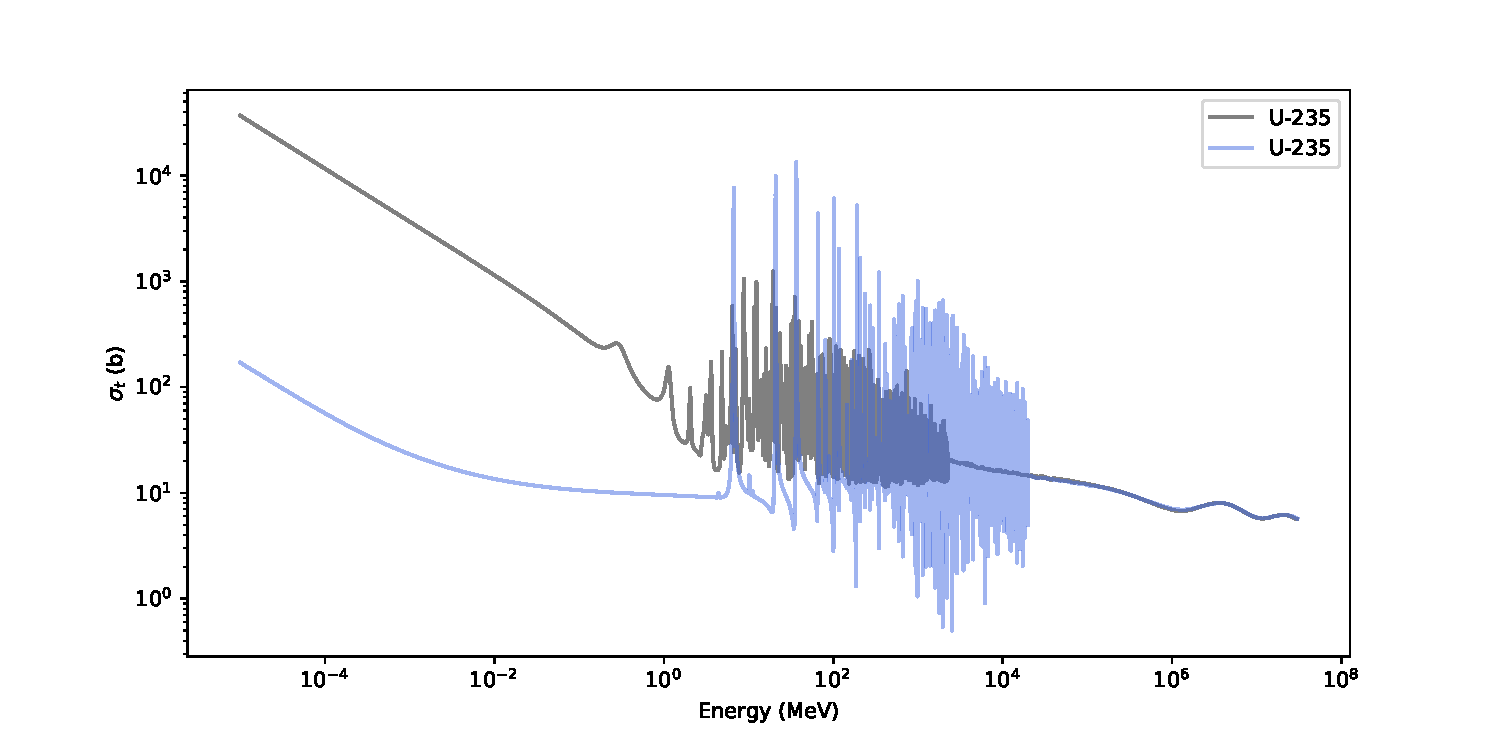
\includegraphics[width=0.85\linewidth]{\figpath/U235-8-XST}
                    \caption{Uranium 235 and 238 total microscopic cross sections as a function of energy. Data provided through the ENDF-8.0 nuclear reaction data library \cite{ENDF8}.}
                    \label{fig:NTT:Cross Section plot}
                \end{figure}

                The complicated dependence on energy would require hundreds of thousands of energy points to faithfully represent for the energies of interest in thermal reactors.
                Modeling of this many energy points in whole-core simulations would require too much memory.
                The multi-group approximation divides this energy space into several energy groups; within each group cross sections are averaged.
                The multi-group eigenvalue transport equation can be found by integrating the \cref{eq:NTT:Eigenvalue Transport Problem} over an energy energy interval $[E_{g}, E_{g-1})$.
                \begin{aequation}\label{eq:NTT:MGEV Transport Problem w/ Anisotropic XS}
                    \left[\dir\vdot\grad + \xst[\loc,\dir]\right]\aflux
                        = \rfourpi\Bigg[&\suml[\gprime=1][G]\intl[\fourpi]\xss[][\loc][\dir,\dirprime]\aflux[\loc][\dirprime][\gprime]\ddirprime \\
                        + &\frac{\spect}{\keff}\suml[\gprime=1][G]\nufis[\loc,\dir]\sflux[\loc]\Bigg]
                \end{aequation}
                \begin{equation*}
                    \forall\loc, \quad \forall\dir\in\fourpi,\quad \forall g\in\{1,2,\ldots,G\},
                \end{equation*}
                where the multi-group quantities are defined by
                \begin{subequations}\label{eqs:NTT:Multi-group Quantities Anisotropic}
                    \begin{equation}\label{eq:NTT:Multi-group Angular Flux}
                        \aflux \defined \intl[E_g][E_{g-1}]\AngularFlux(\loc,\dir,E)\dif{E},
                    \end{equation}
                    \begin{equation}\label{eq:NTT:Multi-group Spectrum}
                        \spect \defined \intl[E_g][E_{g-1}]\Spectrum(\loc,E)\dif{E},
                    \end{equation}
                    \begin{equation}\label{eq:NTT:Multi-group Total Cross Section Anisotropic}
                        \xst[\loc,\dir] \defined \frac{\intl[E_{g}][E_{g-1}]\CrossSection_{t}(\loc,E)\AngularFlux(\loc,\dir,E)\dif{E}}{\aflux},
                    \end{equation}
                    \begin{equation}\label{eq:NTT:Multi-group Fission Cross Section Anisotropic}
                        \nufis[\loc,\dir][g] \defined \frac{\intl[E_{g}][E_{g-1}]\nu\CrossSection_{f}(\loc,E)\AngularFlux(\loc,\dir,E)\dif{E}}{\aflux},
                    \end{equation}
                    \begin{equation}\label{eq:NTT:Multi-group Scattering Cross Section Anisotropic}
                        \xss[][\loc][\dir,\dirprime] \defined \frac{\intl[E_{g}][E_{g-1}]\intl[E_{\gprime}][E_{\gprime-1}]\CrossSection_{s}(\loc,\dirprime\vdot\dir,\Eprime\to E)\AngularFlux(\loc,\dirprime,\Eprime)\dif{\Eprime}\dif{E}}{\aflux[\loc][\dirprime][\gprime]}.
                    \end{equation}
                \end{subequations}

                By defining the cross sections in this way, no approximations have been made, and the reaction rates of each energy group are preserved.
                However, this approach has two issues: the cross sections are dependent on the angular flux which is not known \textit{a priori}, and have dependence on the neutron direction of flight.
                Generally, the dependence on the angular flux is addressed by solving a simplified problem to generate a continuous or fine-group neutron energy spectrum.
                This spectrum is then used to ``collapse'' the cross sections into coarser multi-group values \cite{Knott2010}.
                This introduces approximation into the transport equation.

                To eliminate the directional dependence of the multi-group cross sections, an additional approximation is made: isotropic angular flux spectrum,
                \begin{equation}\label{eq:NTT:Multi-group Isotropic Spectrum}
                    \AngularFlux(\loc,\dir,E) \approx \rfourpi\FluxSpectrum(\loc, E).
                \end{equation}
                Using this approximate angular flux as the weighting function for multi-group cross sections in \cref{eqs:NTT:Multi-group Quantities Anisotropic,eq:NTT:MGEV Transport Problem w/ Anisotropic XS} can be simplified to
                \begin{aequation}\label{eq:NTT:MGEV Transport Problem}
                    \left[\dir\vdot\grad + \xst\right]\aflux = \rfourpi\Bigg[&\suml[\gprime=1][G]\intl[\fourpi]\xss\aflux[\loc][\dirprime][\gprime]\ddirprime\\
                        + \frac{\spect}{\keff}&\suml[\gprime=1][G]\nufis\intl[\fourpi]\aflux[\loc][\dirprime][\gprime]\ddirprime\Bigg],
                \end{aequation}
                \begin{equation*}
                    \forall\loc, \quad \forall\dir\in\fourpi,\quad \forall g\in\{1,2,\ldots,G\},
                \end{equation*}
                where the approximated multigroup cross sections are defined as
                \begin{subequations}\label{eqs:NTT:Multi-group Cross Sections}
                    \begin{equation}\label{eq:NTT:Multi-group Total Cross Section}
                        \xst \defined \frac{\intl[E_{g}][E_{g-1}]\CrossSection_{t}(\loc,E)\FluxSpectrum(\loc,E)\dif{E}}{\intl[E_{g}][E_{g-1}]\FluxSpectrum(\loc,E)\dif{E}},
                    \end{equation}
                    \begin{equation}\label{eq:NTT:Multi-group Fission Cross Section}
                        \nufis[\loc][g] \defined \frac{\intl[E_{g}][E_{g-1}]\nu\CrossSection_{f}(\loc,E)\FluxSpectrum(\loc,E)\dif{E}}{\intl[E_{g}][E_{g-1}]\FluxSpectrum(\loc,E)\dif{E}},
                    \end{equation}
                    \begin{equation}\label{eq:NTT:Multi-group Scattering Cross Section}
                        \xss \defined \frac{\intl[E_{g}][E_{g-1}]\intl[E_{\gprime}][E_{\gprime-1}]\CrossSection_{s}(\loc,\dirprime\vdot\dir,\Eprime\to E)\FluxSpectrum(\loc,\Eprime)\dif{\Eprime}\dif{E}}{\intl[E_{\gprime}][E_{\gprime-1}]\FluxSpectrum(\loc,\Eprime)\dif{\Eprime}}.
                    \end{equation}
                \end{subequations}
            }
            \subsubsection{Spatial Discretization}{\label{sssec:NTT:Spatial Discretization}
                Nearly all computational transport methods involve some form of spatial discretization.
                Reactor designs include many different material regions, and nearly all simulation tools will discretize the spatial domain into these different material regions.
                Deterministic methods will generally apply a finer meshing within these material regions, into transport cells.
                For the purposes of this work, a cell $\mathcal{R}_i$ is indexed with $i$.
                A visualization of the material and hypothetical meshing for a single pin-cell are shown in \cref{fig:NTT:Pin Cell}.
                In deterministic codes, the typical assumption is that material properties (cross sections) are constant within each computational cell.

                \begin{figure}[h]
                    \centering
                    \begin{subfigure}[t]{0.45\linewidth}
                        \centering
                        \def\svgwidth{\linewidth}
                        \input{\figpath/PinCell.pdf_tex}
                        \caption{Material regions}
                        \label{fig:NTT:Pin Cell Materials}
                    \end{subfigure}%
                    \hfill
                    \begin{subfigure}[t]{0.45\linewidth}
                        \centering
                        \def\svgwidth{\linewidth}
                        \input{\figpath/PinCellMesh.pdf_tex}
                        \caption{Hypothetical computational cell mesh}
                        \label{fig:NTT:Pin Cell Mesh}
                    \end{subfigure}
                    \caption{Material and mesh spatial discretization examples for a single pin cell.}
                    \label{fig:NTT:Pin Cell}
                \end{figure}
            }
            \subsubsection{Directional Discretization}{\label{sssec:NTT:Directional Discretization}
                %%% Discrete Ordinates Quantities %%%
\DeclareDocumentCommand{\mprime}{}{m^{\prime}}
\DeclareDocumentCommand{\dirm}{ O{m} }{\dir_{#1}}
\DeclareDocumentCommand{\wt}{ O{m} }{\Weight_{#1}}

% Quadrature set
\DeclareDocumentCommand{\angquad}{ O{N} }{ \mathcal{M}_{#1} }

% Cross-Sections
\DeclareDocumentCommand{\xss}{ o O{\loc} O{ m^{\prime}\!\to m} O{\gprime\!\to g} }{
    \IfNoValueOrEmptyTF{#1}
    {\xs[s,#3][#2][#4]}
    {\xs[s,#1][#2][#4]}
}

% Flux
\DeclareDocumentCommand{\aflux}{ O{\loc} O{m} O{g}}{\ensuremath{\AngularFlux^{#3}_{#2}\!\left(#1\right)}}

% Source
\DeclareDocumentCommand{\source}{ O{\loc} O{m} O{g} }{\ensuremath{q^{#3}_{#2}\!\left(#1\right)}}


                Typically, the directional variable cannot be treated exactly in deterministic methods.
                There are two common methods of approximating behavior as a function of direction $\dir$:
                \begin{enumerate}
                    \item{\ac{PN} Expansion}
                    \item{\ac{SN}}
                \end{enumerate}

                Expansion in spherical harmonics, often referred to as \acs{PN}, is one of the oldest transport methods, where $N$ indicates the order of the expansion.
                In this method, the angular flux is expanded as a linear combination of spherical harmonics moments.
                The simplest expansion of order 1, reduces to the diffusion approximation.

                The \acf{SN} method is a discretization of the directional variable $\dir$; typically, the discrete direction values are determined using a set of quadrature points.
                \begin{subequations}\label{eqs:NTT:Directional Quadrature}
                    Let the $\angquad$ be the set of discrete directions, and weights,
                    \begin{equation}\label{eq:NTT:Directional Quadrature Definition}
                        \angquad \defined \left\{\dirm \in \{\dir_1,\dir_2,\ldots,\dir_N\}, \wt \in \{\wt[1], \wt[2], \ldots,\wt[N]\}\right\},
                    \end{equation}
                    such that a directional integration can be approximated as
                    \begin{equation}\label{eq:NTT:Directional Quadrature Integration}
                        \intl[\fourpi]f(\dir)\ddir \approx \fourpi\suml[m\in\angquad]\wt f(\dirm),
                    \end{equation}
                    where
                    \begin{equation}\label{eq:NTT:Directional Quadrature Weight Sum}
                        \suml[m\in\angquad]\wt = 1.
                    \end{equation}
                \end{subequations}

                There are two common forms of quadrature sets that are commonly used in transport calculations: level-symmetric and product quadratures.
                The level-symmetric quadratures include directions that are evenly distributed over the unit-sphere; this is optimal in situations where each direction has similar variation.
                However, typical reactor designs have significantly less variation in the axial ($z$) direction which fuel rods are oriented along.
                In this situation, neutrons with directions close to the $z$-axis are modeled poorly because there are few azimuthal angles at these polar levels, as is demonstrated in \cref{fig:NTT:S8 Quadrature}.
                These steep polar angles are important in reactor analysis due to self-shielding effects, which are strongly dependent on polar angle. % [CITATION].

                Product quadratures are generated by a multiplicative combination of separate quadrature sets in the azimuthal and polar directions.
                The azimuthal quadrature set in generated over the domain $[0,2\pi]$, while the polar quadrature set is generated for the polar cosine $\mu$ over the domain $[-1,1]$.
                This quadrature generation technique does not suffer from the same issue for steep polar directions, as each polar level has the same number of azimuthal directions.
                A common choice for the azimuthal quadrature generation in the Chebyshev quadrature set, which gives evenly spaced azimuthal angles.
                The polar cosine quadrature set typically uses a Gauss-Legendre quadrature set, or an optimized quadrature set such as the Tabuchi-Yamamoto quadrature \cite{TabuchiYamamotoQuad}.
                \Cref{fig:NTT:ChebyshevGauss Quadrature} shows an example of a product quadrature's set of directions using a Chebyshev azimuthal quadrature and Gauss-Legendre polar quadrature.

                \begin{figure}[h]
                    \centering
                    \begin{subfigure}[t]{0.45\linewidth}
                        \centering
                        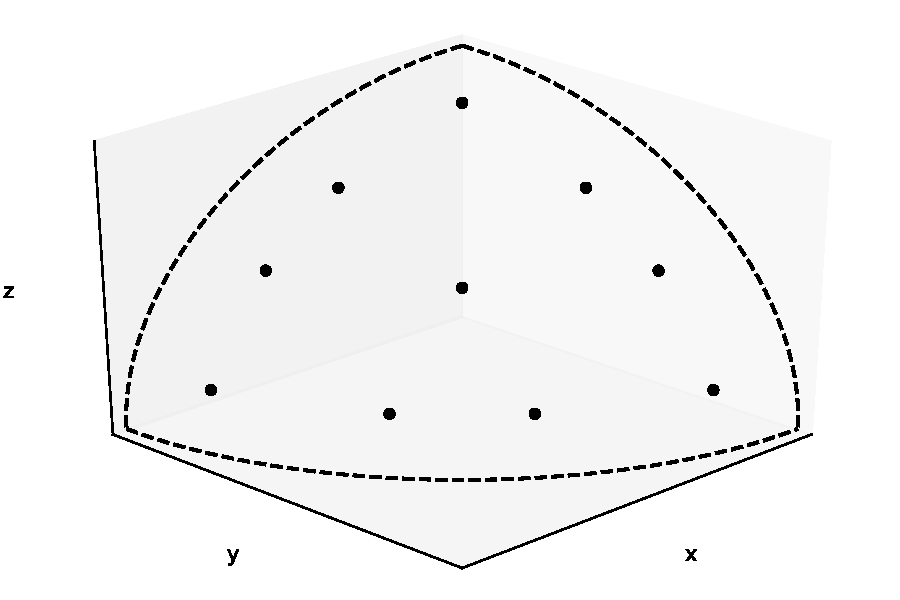
\includegraphics[width=\linewidth]{S8-Quadrature}
                        \caption{Level-Symmetric Quadrature ($S_8$)}
                        \label{fig:NTT:S8 Quadrature}
                    \end{subfigure}%
                    \hfill
                    \begin{subfigure}[t]{0.45\linewidth}
                        \centering
                        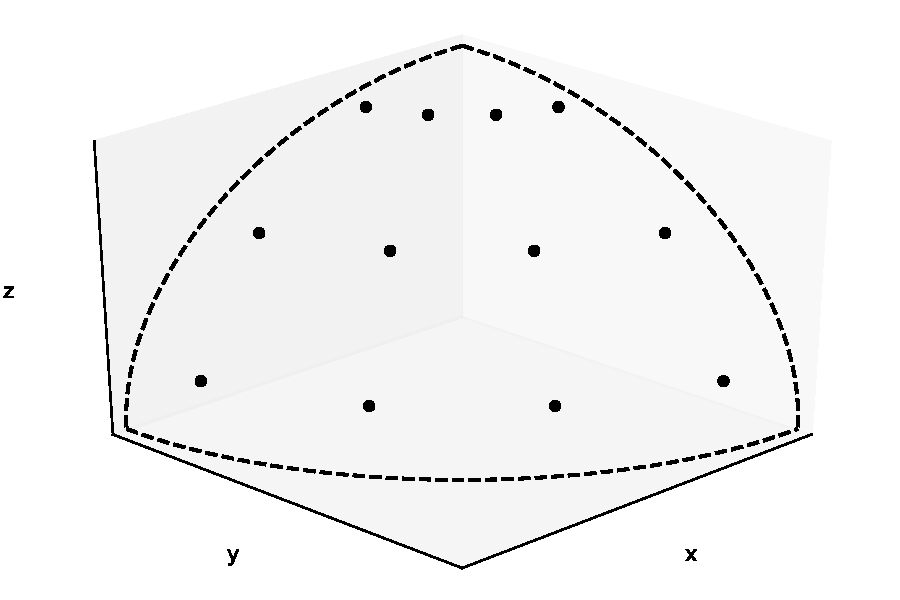
\includegraphics[width=\linewidth]{ChebyshevGauss}
                        \caption{Chebyshev-Gauss Product Quadrature with 4 azimuthal and 3 polar angles}
                        \label{fig:NTT:ChebyshevGauss Quadrature}
                    \end{subfigure}
                    \caption{(a) Level-Symmetric and (b) product quadrature direction set examples shown for a single octant of the unit-sphere.}
                    \label{fig:NTT:Quadrature Examples}
                \end{figure}
            }
            \subsubsection{The Method of Characteristics}{\label{sssec:NTT:MOC}
                The \acf{MOC} is a technique used in mathematics to solve \acp{PDE}, by transforming a \ac{PDE} into a system of \acp{ODE}.
                The method was first applied to the neutron transport problem by \citeauthor{Askew1972} in 1972 \cite{Askew1972}, but only began to see real use in the 1980's \cite{Halsall1980}.
                The \ac{MOC} transforms the transport equation into the characteristic form, by examining the equation along straight neutron paths through the spatial domain.

                Typically, the spatial domain is discretized into cells that have uniform material data (cross sections).
                By examining the equation along one of these characteristic ``tracks'' or ``rays'', the average angular flux along the track within a cell can be calculated.
                The scalar flux can then be found by collecting the average angular flux along all tracks passing through this region, in a numerical integration over space and angle.

                Like the \ac{CP} method, \ac{MOC} is able to handle completely arbitrary geometry; however, it is also able to account for anisotropic scattering.
                Additionally, the \ac{MOC} does not produce the large matrices in realistic applications as the \ac{CP} method does.
                For problems that contain more than a few hundred cells, the \ac{MOC} is generally preferred over \ac{CP} methods \cite{Hebert2010}.

                The \ac{CDP} is a method similar to both \ac{CP} method and the \ac{MOC} \cite{Hong1999,Liu2014}; the major difference from \ac{CP} is that \ac{CDP} only couples together cells are traversed by characteristic tracks.
                This significantly cuts down on the computational resources required by traditional \ac{CP} methods.
                This method has also shown improvements over \ac{MOC} in cases with few unique geometries and constant material properties throughout the simulation; however these conditions are not applicable in problems of interest to industry.

                The \ac{MOC} is the primary subject of this thesis work.
                As such, \cref{ch:The Method of Characteristics} has been devoted to the details of the method, and \cref{ch:Ray-Tracing} expands upon the details of ray-tracing that is central to the \ac{MOC}.
            }
        }
    }
    \section{Source Iteration}{\label{sec:NTT:Source Iteration}
        Generally, the $k$-eigenvalue transport problems, introduced in \cref{sec:NTT:k-Eigenvalue Problems}, are solved iteratively.
        Given an initial guess for the $k$-eigenvalue, boundary conditions, and interior flux-moments, an estimate of the source can be computed.
        A transport ``sweep'' can be performed, in which updated boundary conditions and flux-moments are computed.
        Given these updated flux-moments a new estimate of the eigenvalue can be calculated.
        This process can be repeated until the eigenvalue and flux-moments are converged within some tolerance.
        For simplicity, this process is shown for a isotropic mono-energetic, continuous-space, one-dimensional transport problem in \cref{alg:NTT:Source Iteration}.

        \begin{algorithm}[ht]
            \centering
            \caption{Source Iteration algorithm for the $k$-eigenvalue transport problem.}
            \label{alg:NTT:Source Iteration}
            \begin{algorithmic}[1]
                \State{Begin iteration $j$ with a known boundary conditions, scalar flux estimate, $\ScalarFlux^{(j)}(x)$, and a $k$-eigenvalue estimate, $\keff^{j}$.}
                \State{Perform a transport sweep:
                    \begin{equation}\label{eq:NTT:Source Iteration:Transport Sweep}
                        \left[\PolarCos\pderiv{}{x} + \CrossSection_t(x)\right]\AngularFlux^{(j+1)}(x,\PolarCos) = \frac{1}{2}\left[\CrossSection_s(x) + \frac{1}{\keff^{(j)}}\nu\CrossSection_f(x)\right]\ScalarFlux^{(j)}(x),
                    \end{equation}
                    \begin{equation*}
                        \forall x\in [0,X], \quad \forall\PolarCos \in [-1, 1].
                    \end{equation*}
                }
                \State{Update the scalar flux, and the eigenvalue for the next iteration:
                    \begin{subequations}\label{eqs:NTT:Source Iteration:Update}
                        \begin{equation}\label{eq:NTT:Source Iteration:Scalar Flux Update}
                            \ScalarFlux^{(j+1)}(x) = \intl[-1][1]\AngularFlux^{(j+1)}(x,\PolarCos)\dif{\PolarCos} \frac{\Phi_0}{\frac{1}{X}\intl[0][X]\intl[-1][1]\AngularFlux^{(j+1)}(x',\PolarCos)\dif{\PolarCos}\dif{x'}},
                        \end{equation}
                        \begin{equation}\label{eq:NTT:Source Iteration:Eigenvalue Update}
                            \keff^{(j+1)} = \frac{\intl[0][X]\nu\CrossSection_f\ScalarFlux^{(j+1)}(x)\dif{x}}{\intl[0][X]\CrossSection_a\ScalarFlux^{(j+1)}(x)\dif{x}}.
                        \end{equation}
                    \end{subequations}
                }
                \State{Repeat steps 1. - 3. until sufficient convergence.}
            \end{algorithmic}
        \end{algorithm}

        \subsection{Transport Acceleration}{\label{ssec:NTT:Transport Acceleration}
            While \cref{alg:NTT:Source Iteration} is valid, it typically converges very slowly, requiring many iterations to get reasonable results.
            In full-core calculations, a single transport sweep can become computationally expensive and using \cref{alg:NTT:Source Iteration} is not feasible.
            There has been considerable effort in developing methods that accelerate transport calculations by using a lower-order calculation, typically based on the diffusion approximation.
            These method reduce the spectral radius of the iteration scheme, and thus fewer transport iterations are necessary to provide converged results.

            While other acceleration methods exist \cite{Hebert2017}, the most common are \ac{NDA} methods \cite{Smith2002}, typically using the \ac{CMFD} method \cite{Smith1983}.
            \Cref{alg:NTT:NDA} lists the standard \ac{NDA} algorithm for a 1-D mono-energetic $k$-eigenvalue problem.
            The primary difference between \ac{CMFD} and \ac{NDA} is that \ac{CMFD} uses a coarser mesh than the transport problem, while \ac{NDA} uses the same mesh as the transport problem.

            The \ac{CMFD} acceleration method has been shown to significantly reduce computational transport run-times \cite{Smith2002,Anistratov2011,Collins2016}.
            Improvements upon the original \ac{CMFD} formulation \cite{Smith1983}, such as p\ac{CMFD} \cite{Cho2002} and od\ac{CMFD} \cite{Zhu2016}.
            The p\ac{CMFD} method preserves partial currents rather than net currents, and has been shown to be unconditionally stable for transport problems at fixed conditions \cite{Cho2002}.
            The od\ac{CMFD} method generalizes the \ac{CMFD} and p\ac{CMFD} methods by adding an artificial term to the diffusion coefficient, and has faster convergence properties than p\ac{CMFD} \cite{Zhu2016}.

            Utilization of \ac{CMFD} acceleration in transport calculations with \ac{TH} feedback has not had the favorable stability and convergence properties as calculations without feedback \cite{Kochunas2017}.
            Many transport codes have required under-relaxation of the scalar flux in the iteration schemes for stability in these calculations; there is ongoing research investigating a less ad-hoc approach \cite{Kochunas2017}.
            This instability and convergence slow-down in problems with feedback has prevented full utilization of more advanced multi-level solvers \cite{Kochunas2017,Yee2018a}.

            \begin{algorithm}
              \caption{\ac{NDA} Acceleration algorithm for the $k$-eigenvalue transport problem.}
              \label{alg:NTT:NDA}
              \newcommand{\ndaCurrent}[1][j]{J^{(#1)}(x)}
              \newcommand{\ndaFlux}[1][j]{\ScalarFlux^{(#1)}(x)}
              \newcommand{\ndaXST}{\CrossSection_{t}(x)}
              \newcommand{\ndaXSA}{\CrossSection_{a}(x)}
              \newcommand{\ndaNUFIS}{\nu\CrossSection_{f}(x)}
              \newcommand{\ndaD}{\frac{1}{3\ndaXST}}
              \newcommand{\ndaDHAT}{\widehat{D}^{(j)}(x)}

              \begin{algorithmic}[1]
                \State{Begin iteration $i$ with known boundary conditions, scalar flux estimate, $\ScalarFlux^{(j)}(x)$, a net current estimate, $\Current^{(j)}(x)$, and a $k$-eigenvalue estimate, $\keff$.}
                \State{Compute linear and non-linear correction factors for low-order diffusion equation:
                  \begin{equation}\label{eq:NTT:NDA:Dhat}
                    \ndaDHAT = \frac{\deriv{}{x}\left[\ndaCurrent + \ndaD\deriv{\ndaFlux}{x}\right]}{\ndaFlux}
                  \end{equation}
                }
                \State{Solve the low-order diffusion eigenvalue problem:
                  \begin{equation}\label{eq:NTT:NDA:NDA Equation}
                    -\deriv{}{x}\ndaD\deriv{\ndaFlux[j+1/2]}{x}
                    +\left[\ndaXSA + \ndaDHAT\right]\ndaFlux[j+1/2] = \frac{1}{\keff}\ndaNUFIS\ndaFlux[j+1/2].
                  \end{equation}
                }
                \State{Perform a transport sweep using the scalar flux, and eigenvalue estimates from the low-order diffusion calculation:
                  \begin{equation}\label{eq:NTT:NDA:Transport Sweep}
                    \left[\PolarCos\pderiv{}{x} + \ndaXST\right]\AngularFlux^{(j+1)}(x,\PolarCos) = \frac{1}{2}\left[\CrossSection_s(x) + \frac{1}{\keff^{(j)}}\nu\CrossSection_f(x)\right]\ScalarFlux^{(j)}(x),
                  \end{equation}
                  \begin{equation*}
                      \forall x\in [0,X], \quad \forall\PolarCos \in [-1, 1].
                  \end{equation*}
                }
                \State{Update the scalar flux, current, and eigenvalue estimates for next iteration:
                  \begin{subequations}\label{eqs:NTT:NDA:Update}
                    \begin{equation}\label{eq:NTT:NDA:Scalar Flux Update}
                      \ScalarFlux^{(j+1)}(x) = \intl[-1][1]\AngularFlux^{(j+1)}(x,\PolarCos)\dif{\PolarCos} \frac{\Phi_0}{\frac{1}{X}\intl[0][X]\intl[-1][1]\AngularFlux^{(j+1)}(x',\PolarCos)\dif{\PolarCos}\dif{x'}},
                    \end{equation}
                    \begin{equation}\label{eq:NTT:NDA:Current Update}
                      \Current^{(j+1)}(x) = \intl[-1][1]\PolarCos\AngularFlux^{(j+1)}(x,\PolarCos)\dif{\PolarCos} \frac{\Phi_0}{\frac{1}{X}\intl[0][X]\intl[-1][1]\AngularFlux^{(j+1)}(x',\PolarCos)\dif{\PolarCos}\dif{x'}},
                    \end{equation}
                    \begin{equation}\label{eq:NTT:NDA:Eigenvalue Update}
                      \keff^{(j+1)} = \frac{\intl[0][X]\nu\CrossSection_f\ScalarFlux^{(j+1)}(x)\dif{x}}{\intl[0][X]\CrossSection_a\ScalarFlux^{(j+1)}(x)\dif{x}}.
                    \end{equation}
                  \end{subequations}
                }
              \end{algorithmic}
            \end{algorithm}
        }
    }

    % References
    \printbibliography
}